\documentclass{standalone}
%\documentclass[a4paper]{article}
%\usepackage{geometry}
\usepackage{tikz}

\begin{document}

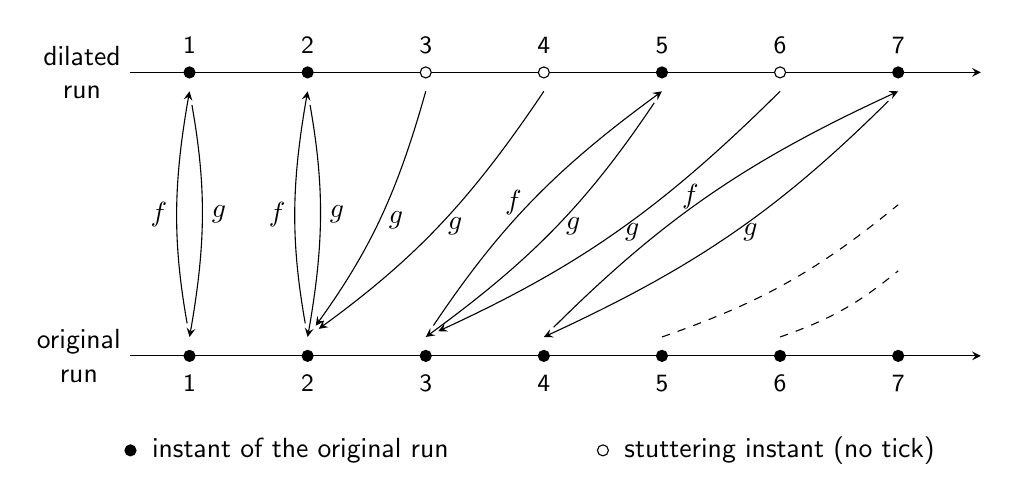
\begin{tikzpicture}[>=stealth,x=1.5cm,y=1.2cm]
	\sffamily
	\draw[->] (0.5,0) -- ++(7.2,0) ;
	\node[left, align=center] at (0.5,0) {original\\run} ;
	\node[left, align=center] at (0.5,3) {dilated\\run} ;
	\draw[->] (0.5,3) -- ++(7.2,0) ;
	\foreach \x in {1,...,7} {
		\draw[fill=black] (\x,0) circle[radius=0.07cm] ;
		\node[below] at (\x,-0.1) {\small\x} ;
		\node[above] at (\x,3.1) {\small\x} ;
	}
	\foreach \x in {1,2,    5,  7} \draw[fill=black] (\x,3.0) circle[radius=0.07cm] ;
	\foreach \x in {    3,4,  6  } \draw[fill=white] (\x,3.0) circle[radius=0.07cm] ;

	\foreach \x / \z in {1 / 1, 2 / 2, 3 / 5, 4 / 7} {
		\draw[->,shorten <=5pt] (\x,0.2) to[bend left=10] node[left,midway] {\(f\)} (\z, 2.8);
		\draw[<-,shorten >=5pt] (\x,0.2) to[bend right=10] node[right,midway] {\(g\)} (\z, 2.8);
  }
	\foreach \x / \z in {2 / 3, 2 / 4, 3 / 6} {
		\draw[<-,shorten <=5pt] (\x,0.2) to[bend right=10] node[right,midway] {\(g\)} (\z, 2.8);
  }
	\draw[dashed] (5,0.2) to [bend right=10] (7,1.6) ;
	\draw[dashed] (6,0.2) to [bend right=10] (7,0.9) ;
	
	\draw[fill=black] (0.5,-1) circle[radius=0.07cm] ;
	\node[right] at (0.6,-1) {instant of the original run} ;
	\draw[fill=white] (4.5,-1) circle[radius=0.07cm] ;
	\node[right] at (4.6,-1) {stuttering instant (no tick)} ;
\end{tikzpicture}

\end{document}
